%Configuracion del tipo de documento, los margenes, la sangria y el interlineado
\documentclass[12pt, a4paper]{report}
\usepackage[top=2.5cm, bottom=2.5cm, left=3cm,right=2.5cm]{geometry}
\usepackage{setspace} %colocar interlineado
\spacing{1.5} % interlineado 1.5
\setlength{\parindent}{1cm} % sangria
\setlength{\parskip}{\baselineskip} %espacio entre parrafos
\usepackage{microtype} %realiza micro-arreglos en los parrafos para que queden mas justificados
\renewcommand{\rmdefault}{phv} % Arial
\renewcommand{\sfdefault}{phv} % Arial
\usepackage{placeins} % ayuda a que las tablas no queden en medio de los textos
\usepackage{tabulary} %tabla que ajusta celdas al texto
\usepackage[font={footnotesize}]{caption} % tamano para la descripcion de las tablas
\captionsetup{labelformat=empty} % elimina el prefijo de los nombres de las tablas
\usepackage{array}
\usepackage{float}
\usepackage{makecell}
\usepackage{graphicx}
\usepackage[spanish,es-tabla,english]{babel}
\usepackage[authoryear,datebegin]{flexbib}
\bibliographystyle{flexbib}

\newcommand{\membrete}{
	
\includegraphics[width=0.15\textwidth]{./img/logo-uc.png}~\\[1cm]

	\textsc{ UNIVERSIDAD DE CARABOBO \\	
	Facultad Experimental de Ciencias y Tecnolog\'{i}a\\
	Departamento de Computaci\'{o}n
	}
}

\newcommand{\titulo}{SOFTWARE PARA EL ESPECTROFOT\'{O}METRO MINISCAN XE PLUS USADO EN EL DIAGN\'{O}STICO DE PATOLOG\'{I}AS DERMATOL\'{O}GICAS EN PACIENTES. CASO DE ESTUDIO: CIMBUC.}

\makeatletter
\renewcommand{\@chapapp}{Cap\'{i}tulo}% Not necessary...
\newenvironment{chapquote}[2][2em]
  {\setlength{\@tempdima}{#1}%
   \def\chapquote@author{#2}%
   \parshape 1 \@tempdima \dimexpr\textwidth-2\@tempdima\relax%
   \itshape}
  {\par\normalfont\hfill--\ \chapquote@author\hspace*{\@tempdima}\par\bigskip}
\makeatother

\begin{document}
	\selectlanguage{spanish}
	\begin{titlepage}
	\begin{center}
	\membrete
	\vfill
	\titulo
	\vfill
	% Autor y Tutores
	\textbf{AUTOR:}\\
	Gabriel N\'{u}\~{n}ez

	\textbf{TUTORES:} \\
	Prof. Patricia Guerrero \\
	Prof. Harold Vasquez
	\vfill
	Naguanagua, \today
	\end{center}
\end{titlepage}
	\renewenvironment{abstract}{
  \vspace*{\fill}
  \begin{center}%
    \bfseries\abstractname
  \end{center}}%

\begin{abstract}
	\noindent
El espectrofot\'{o}metro de reflexi\'{o}n difusa, denominado MiniScan XE Plus, es un instrumento de medici\'{o}n utilizado por el Centro de Investigaciones M\'{e}dicas y Biotecnol\'{o}gicas de la Universidad de Carabobo (CIMBUC), que ayuda a los dermat\'{o}logos a establecer diagn\'{o}sticos sobre patolog\'{i}as en la piel de pacientes, de manera precisa y sin necesidad de realizar biopsias. No obstante, el software comercial disponible para la utilizaci\'{o}n de tal instrumento es poco amigable, dif\'{i}cil de utilizar e imposible de modificar y extender. La presente investigaci\'{o}n tiene como objetivo desarrollar un software amigable, modificable y extensible, que se ajuste a las necesidades de los dermat\'{o}logos y que garantice un mejor aprovechamiento del instrumento en cuesti\'{o}n.

	\noindent
	\textbf{Palabras claves:} espectrofot\'{o}metro, an\'{a}lisis bioqu\'{i}mico de la piel, biopsia, software privativo, software libre.
	\vfill
\end{abstract}

\vfill

\selectlanguage{english}
\begin{abstract}
	\noindent
The diffuse reflectance spectrophotometer, called MiniScan XE Plus, is a measurement instrument used by the Medical Research and Biotechnology Center at the University of Carabobo (CIMBUC), which helps dermatologists to establish pathologies diagnoses in the skin of patients precisely, without need for biopsy. However, the available commercial software for the use of such an instrument is unfriendly, difficult to use and impossible to modify and extend. This research aims to develop a friendly, modifiable and expandable software that meets the needs of dermatologists and ensures a better use of the instrument itself.

	\noindent
	\textbf{Keywords:} spectrophotometer, biochemical analysis of the skin, biopsy, privative software, open source software.
	\vfill
\end{abstract}

\selectlanguage{spanish}
	\newpage
	\chapter{\label{cap:1}El Problema}

	\section{Planteamiento del Problema}	
\cite{Bersha} indica que durante el diagn\'{o}stico de enfermedades de la piel, la observaci\'{o}n cuidadosa y la evaluaci\'{o}n visual del \'{a}rea sospechada es siempre el primer paso y el m\'{a}s importante. Esto es seguido generalmente por una escisi\'{o}n o biopsia por punci\'{o}n, en la que se extrae una muestra de tejido de la piel para un an\'{a}lisis microsc\'{o}pico. La observaci\'{o}n visual suele ser subjetiva y los pacientes a menudo se someten a cicatrices y dolor durante la escisi\'{o}n. Por otro lado, las t\'{e}cnicas \'{o}pticas son por lo general no invasivas y los resultados de estas son a menudo objetivos. Durante el diagn\'{o}stico no invasivo no se crea ninguna ruptura en la piel, y los pacientes no se someten al dolor y a cicatrices durante el tratamiento.

Los avances tecnol\'{o}gicos en la actualidad permiten emplear t\'{e}cnicas de \'{o}ptica con la capacidad de estudiar  las propiedades estructurales y bioqu\'{i}micas del tejido biol\'{o}gico de manera precisa y no invasiva. Los instrumentos que emplean tales t\'{e}cnicas son de gran ayuda para los m\'{e}dicos dermat\'{o}logos, raz\'{o}n por la cual han tomado suma importancia en el \'{a}rea m\'{e}dica dermatol\'{o}gica.

Hoy d\'{i}a existen diferentes tipos de estudios \'{o}pticos in-situ, in-vivo e invitro del tejido biol\'{o}gico, como lo es la espectroscop\'{i}a de reflectancia difusa. Con esta t\'{e}cnica es  posible estudiar las propiedades bioqu\'{i}micas y las condiciones estructurales de un tejido biol\'{o}gico, analizando la interacci\'{o}n luz-tejido de una manera no invasiva \cite{Perez-Gallardo}.

En este sentido, el Centro de Investigaciones M\'{e}dicas y Biotecnol\'{o}gicas de la Universidad de Carabobo (CIMBUC) dispone de un Espectrofot\'{o}metro de reflexi\'{o}n difusa denominado ``MiniScan XE Plus''. La empresa ``HunterLab'', creadora y distribuidora del ``MiniScan XE Plus'', lo describe como un instrumento utilizado para medir la transmisi\'{o}n y/o reflectancia de espec\'{i}menes, como una funci\'{o}n de longitud de onda, que aplica una t\'{e}cnica llamada espectroscop\'{i}a de reflectancia difusa. 

Ahora bien, para emplear el uso del instrumento en estudio, el CIMBUC ha tenido que utilizar el software comercial disponible para la utilizaci\'{o}n del mismo, denominado ``HunterLab Universal Software'', el cual es un software propietario de 16-bit dise\~{n}ado para el Sistema Operativo Microsoft Windows Version 3.x, con la posibilidad de ejecutarse en Windows 95, Windows 2000 y Windows NT, y el mismo fue descontinuado en el a\~{n}o 2008. Este software ofrece un conjunto de funcionalidades que abarcan no s\'{o}lo la utilizaci\'{o}n del Espectrofot\'{o}metro, sino tambi\'{e}n la utilizaci\'{o}n de otros instrumentos ofrecidos por la empresa ``HunterLab''. La interfaz gr\'{a}fica de usuario de dicho software esta en idioma ingl\'{e}s. Por \'{u}ltimo, los resultados que genera este software no poseen el formato de gesti\'{o}n de informaci\'{o}n de pacientes con el que trabajan los dermat\'{o}logos del CIMBUC.

Tomando en cuenta lo mencionado anteriormente se tiene que el software comercial es propietario y est\'{a} descontinuado, por lo tanto no existe la posibilidad de modificarlo, mejorarlo ni extenderlo; ofrece funcionalidades ajenas al uso exclusivo del Espectrofot\'{o}metro, causando que la interfaz gr\'{a}fica de usuario contenga m\'{a}s opciones disponibles de las necesarias para manejar el instrumento en estudio. Asimismo, como consecuencia de que la interfaz gr\'{a}fica de usuario est\'{e} en idioma ingl\'{e}s, \'{e}sta es dif\'{i}cil de entender por los dermat\'{o}logos. Aunado al hecho de que los resultados generados por dicho software no poseen el formato con el que trabajan los dermat\'{o}logos, haciendo necesario su traspaso manual, lo que produce a una ralentizaci\'{o}n en las consultas con pacientes. Todo esto conlleva a que los m\'{e}dicos requieran de asistencia t\'{e}cnica entrenada, disponible en todo momento para guiar el uso apropiado del software.

De lo antedicho se desprende que, el software comercial en utilizaci\'{o}n para el manejo del Espectrofot\'{o}metro posee una interfaz gr\'{a}fica de usuario poco amigable, y el costo del tiempo de capacitaci\'{o}n para su uso correcto podr\'{i}a ser alto. \'{E}ste software no podr\'{a} modificarse, mejorarse ni extenderse por el hecho de ser propietario, y por lo tanto no se fomentar\'{a} el uso del instrumento en cuesti\'{o}n en el campo m\'{e}dico (p\'{u}blico o privado). De igual manera, tampoco se fomentar\'{a} el desarrollo de nuevas aplicaciones que utilicen sus resultados como insumo, sosegando as\'{i} la posibilidad de realizar an\'{a}lisis m\'{a}s complejos y de proveer a los dermat\'{o}logos de resultados que les permitan establecer diagn\'{o}sticos m\'{a}s completos.

Motivado a todo lo anterior, se desarroll\'{o} un nuevo software para el Espectrofot\'{o}metro, con una interfaz gr\'{a}fica de usuario amigable, utilizando los lineamientos de la ingenier\'{i}a del software pertinentes y favoreciendo su integraci\'{o}n con nuevas aplicaciones que se desarrollen en proyectos futuros, logrando as\'{i} el nivel deseado de amigabilidad y extensibilidad.

Con esta investigaci\'{o}n se espera fomentar la utilizaci\'{o}n del nuevo software, una mejor capacitaci\'{o}n del personal m\'{e}dico para su debido uso y el aporte de una base s\'{o}lida sobre la cual se podr\'{a}n desarrollar nuevos proyectos.

	\section{Justificaci\'{o}n}
El estudio y diagn\'{o}stico de patolog\'{i}as dermatol\'{o}gicas en pacientes es un \'{a}rea cuyo campo est\'{a} en constante desarrollo, requiriendo que los procesos involucrados en \'{e}sta no solamente sean de calidad, sino que sean capaces de desarrollarse a la par; el software utilizado en dicha \'{a}rea no es una excepci\'{o}n. Que los dermat\'{o}logos experimenten dificultades al momento de utilizar el ``HunterLab Universal Software'' debido a que el mismo este en ingl\'{e}s, ofrezca funciones ajenas al instrumento en estudio, no emplee el formato de historia m\'{e}dica utilizado por ellos, y que adem\'{a}s no ofrezca la posibilidad de modificarlo, mejorarlo ni agregarle nuevas funciones, es un problema grave, ya que no s\'{o}lo ralentiza cada consulta con un paciente, sino que genera la necesidad de asistencia t\'{e}cnica disponible en todo momento para la debida utilizaci\'{o}n de dicho software; por \'{u}ltimo y no menos importante, disminuye el nivel de aprovechamiento potencial del instrumento de medici\'{o}n en estudio.

Con respecto a software de calidad, \cite{Sommerville} explica lo siguiente: As\'{i} como los servicios que proveen, los productos de software tienen cierto n\'{u}mero de atributos asociados que reflejan la calidad de ese software. Estos atributos no est\'{a}n directamente relacionados con lo que el software hace. M\'{a}s bien, reflejan su comportamiento durante su ejecuci\'{o}n, en la estructura y organizaci\'{o}n del programa fuente, y en la documentaci\'{o}n asociada. Ejemplos de estos atributos son el tiempo de respuesta del software a una pregunta del usuario y la comprensi\'{o}n del programa fuente.

El conjunto espec\'{i}fico de atributos que se espera de un software depende obviamente de su aplicaci\'{o}n. Esto se generaliza en el conjunto de atributos que se muestran en la Tabla 1, la cual contiene las caracter\'{i}sticas esenciales de un software bien dise\~{n}ado.

	\begin{table}[htb]
		\small
		\centering
		\setlength{\extrarowheight}{5pt}
		\begin{tabulary}{15cm}{|c|L|}
			\hline
			\textbf{Caracter\'{i}stica} & \textbf{Descripci\'{o}n}\\ \hline
			\textbf{Mantenibilidad} & El software debe describirse de tal forma que pueda evolucionar  para cumplir las necesidades de cambio de los 					clientes. Este es un atributo cr\'{i}tico, debido a que el cambio en el software es una consecuencia inevitable de un cambio en el entorno de negocios.\\ \hline
			\textbf{Confiabilidad} & La confiabilidad del software tiene un gran n\'{u}mero de caracter\'{i}sticas, incluyendo la fiabilidad, protecci\'{o}n y seguridad. El software confiable no debe causar da\~{n}os f\'{i}sicos o econ\'{o}micos en el caso de una falla del sistema.\\ \hline
			\textbf{Eficiencia} & El software no debe hacer que se malgasten los recursos del sistema, como la memoria y los ciclos de procesamiento. Por lo tanto, la eficiencia incluye tiempos de respuesta y de procesamiento, utilizaci\'{o}n de la memoria, etc\'{e}tera.\\ \hline
			\textbf{Usabilidad} & El software debe ser f\'{a}cil de utilizar, sin esfuerzo adicional por el usuario para quien est\'{a} dise\~{n}ado. Esto significa que debe tener una interfaz gr\'{a}fica de usuario apropiada y una documentaci\'{o}n adecuada.\\ \hline
		\end{tabulary}
			\caption{\textbf{Tabla 1.} \textit{Atributos esenciales de un buen software}		(Fuente: Sommerville, 2005).}
	\end{table}
			\FloatBarrier %you shall not pass table!!
Debido a que el ``HunterLab Universal Software'' es propietario, el CIMBUC no dispone del c\'{o}digo fuente del mismo, lo que se traduce en la inexistencia del primer atributo esencial para un buen software: la mantenibilidad; ya que el software propietario no puede ser cambiado ni adaptarse a necesidades espec\'{i}ficas. Por la misma raz\'{o}n de ser un software propietario del cual no se tiene el c\'{o}digo fuente, no se puede determinar con certidumbre el segundo atributo: la confiabilidad; debido a que no se puede evaluar completamente el nivel de protecci\'{o}n y seguridad existentes en dicho software. Por \'{u}ltimo y no menos importante, la usabilidad del software existente es baja, ya que la interfaz gr\'{a}fica de usuario es poco amigable, haciendo surgir la necesidad de disponer de personal t\'{e}cnico para la utilizaci\'{o}n correcta del mismo. Por estas razones, se desarroll\'{o} un software que cumpliese con los atributos esenciales que debe poseer un buen software.

\cite{Sommerville} se\~{n}ala que un dise\~{n}o cuidadoso de la interfaz gr\'{a}fica de usuario es parte fundamental del proceso de dise\~{n}o general del software. Si un software debe alcanzar su potencial m\'{a}ximo, es fundamental que su interfaz gr\'{a}fica de usuario sea dise\~{n}ada para ajustarse a las habilidades, experiencia y expectativas de sus usuarios previstos. Un buen dise\~{n}o de la interfaz gr\'{a}fica de usuario es cr\'{i}tico para la confiabilidad del software. Muchos de los llamados ``errores de usuario'' son causados por el hecho de que las interfaces gr\'{a}ficas de usuario no consideran las habilidades de los usuarios reales y su entorno de trabajo.

El dise\~{n}o de la interfaz gr\'{a}fica de usuario del ``HunterLab Universal Software'' es la principal raz\'{o}n por la cual los dermat\'{o}logos requieren de personal t\'{e}cnico que los asista al momento de utilizarlo. Esto porque dicha interfaz est\'{a} en idioma ingl\'{e}s, contiene funcionalidades que no son necesarias para la utilizaci\'{o}n de Espectrofot\'{o}metro y no proporciona el formato con el que trabajan los dermat\'{o}logos, lo que dificulta la utilizaci\'{o}n de dicha interfaz. Por estas razones los dermat\'{o}logos perciben este software comercial como no intuitivo, ni auto descriptivo ni amigable, temiendo cometer errores al utilizarlo por su propia cuenta y generar resultados err\'{o}neos, poniendo en riesgo el diagn\'{o}stico, y en consecuencia, la salud de los pacientes en consulta.

En conclusi\'{o}n, siguiendo los lineamientos de dise\~{n}o y calidad del software que se consideraron pertinentes, se desarroll\'{o} un software amigable, modificable y extensible, el cual ofrece las funciones que necesitan los dermat\'{o}logos para establecer diagn\'{o}sticos, emplea el formato de historia m\'{e}dica con el que trabajan, permite la exportaci\'{o}n de los resultados a un formato de archivo portable; por \'{u}ltimo y no menos importante, se cre\'{o} una base sobre la cual se prodr\'{a}n trabajar proyectos futuros que necesiten utilizar los resultados de este software como insumo.
	\newpage

	\section{Objetivos de la Investigaci\'{o}n}
En la siguiente secci\'{o}n se especifican los objetivos del trabajo, distinguiendo entre el objetivo general y los objetivos espec\'{i}ficos.
		\subsection{Objetivo General}
	Desarrollar un software para el Espectrofot\'{o}metro ``MiniScan XE Plus'', usado en el diagn\'{o}stico de patolog\'{i}as dermatol\'{o}gicas en pacientes, tomando como caso de estudio el CIMBUC.
		\subsection{Objetivos Espec\'{i}ficos}
			\begin{itemize}
				\item Investigar el estado del arte referente a las caracter\'{i}sticas de software para Espectrofot\'{o}metros de reflexi\'{o}n difusa, dise\~{n}o y calidad de software.
				\item Seleccionar una metodolog\'{i}a que gu\'{i}e el dise\~{n}o y desarrollo del nuevo software para el Espectrofot\'{o}metro ``MiniScan XE Plus''.
				\item Dise\~{n}ar el nuevo software siguiendo la metodolog\'{i}a seleccionada.
				\item Desarrollar el nuevo software, siguiendo la metodolog\'{i}a seleccionada.
				\item Dise\~{n}ar las pruebas para el nuevo software.
				\item Elaborar el manual de usuario del nuevo software.
			\end{itemize}
	\newpage
	\chapter{\label{cap:2}Marco Te\'{o}rico}

	\section{Antecedentes}	
		\begin{itemize}
			\item Por agregar.
		\end{itemize}

	\section{Observaci\'{o}n Directa}
		\begin{itemize}
			\item \textbf{HunterLab Universal Software:} Es un software propietario de 16-bit dise\~{n}ado para el Sistema Operativo Microsoft Windows Version 3.x, con la posibilidad de ejecutarse en Windows 95, Windows 2000, Windows NT y Windows XP, descontinuado en el a\~{n}o 2008. Este software dispone de algunas de funcionalidades desarrolladas en el nuevo software, raz\'{o}n por la cual es una importante referencia.
		
			\item \textbf{MiniScanXE Plus OCX Kit:} Es un archivo de control ActiveX dise\~{n}ado por HunterLab para controlar y/o realizar mediciones con el ``MiniScan XE Plus'', utilizando Visual Basic for Applications (VBA). Su principal objetivo es proveer a los desarrolladores con un componente reutilizable de software que da acceso a las caracteristicas m\'{a}s comunmente utilizadas por el instrumento. La interfaz p\'{u}blica que expone este archivo es utilizada para realizar la comunicaci\'{o}n entre el ``MiniScan XE Plus'' y el nuevo software.
		\end{itemize}
	\newpage
	\chapter{\label{cap:3}Marco Metodol\'{o}gico}

	\section{Metodolog\'{i}a Investigaci\'{o}n-Acci\'{o}n}
	\cite{Baskerville} define la Investigaci\'{o}n-Acci\'{o}n como un m\'{e}todo de investigaci\'{o}n que a finales de la d\'{e}cada de los 90 empez\'{o} a crecer en popularidad, para el uso en investigaciones acad\'{e}micas de sistemas de informaci\'{o}n. Este m\'{e}todo produce resultados de investigaci\'{o}n altamente relevantes, debido a que se fundamenta en la acci\'{o}n pr\'{a}ctica, dirigida a resolver un problema mientras se informa cuidadosamente sobre la teor\'{i}a.

	Esta metodolog\'{i}a tiene una doble finalidad: generar un beneficio al cliente de la investigaci\'{o}n y al mismo tiempo, generar conocimiento de investigaci\'{o}n relevante. Por lo tanto, es una forma de investigar de car\'{a}cter colaborativo que busca unir teor\'{i}a y la pr\'{a}ctica entre investigadores y practicantes, mediante un proceso de naturaleza c\'{i}clica.

	La representaci\'{o}n m\'{a}s habitual de la Investigaci\'{o}n-Acci\'{o}n es la descrita por \cite{Baskerville}, en forma de cinco fases que conforman un ciclo, las cuales se describen en la Figura 1.

\FloatBarrier %you shall not pass table!!
\vline
	\begin{figure}
		\centering
		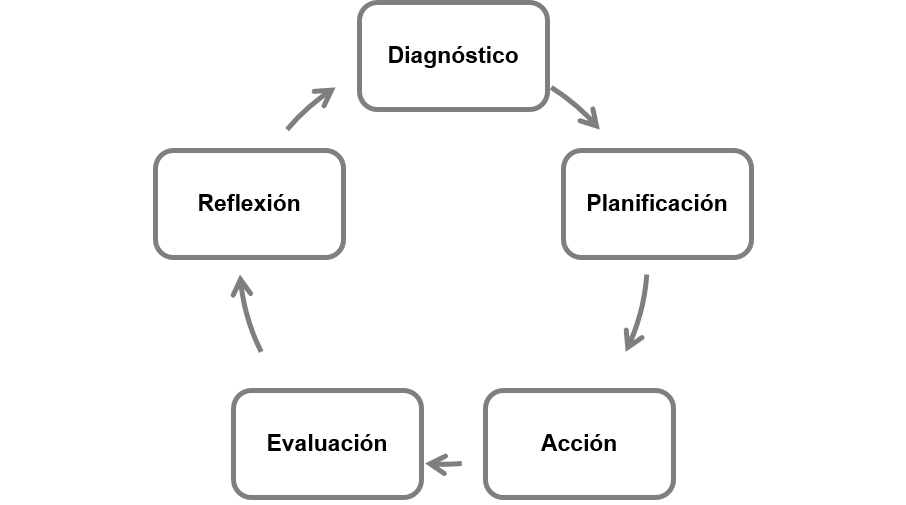
\includegraphics[scale=0.77]{img/investigacion-accion.png}
			\caption{\textbf{Figura 1.} \textit{Car\'{a}cter c\'{i}clico de Investigaci\'{o}n-Acci\'{o}n} (Fuente: Baskerville, 1999).}
	\end{figure}
\FloatBarrier %you shall not pass table!!

	\begin{itemize}
		\item \textbf{Fase de diagn\'{o}stico:} se realiza el proceso de identificaci\'{o}n de los problemas primarios de la investigaci\'{o}n.
		\item \textbf{Fase de planificaci\'{o}n:} se especifican las acciones que se llevaran a cabo para solucionar los problemas primarios.
		\item \textbf{Fase de acci\'{o}n:} se ejecutan las acciones planificadas en la fase anterior.
		\item \textbf{Fase de evaluaci\'{o}n u observaci\'{o}n:} se efect\'{u}a una evaluaci\'{o}n de los resultados obtenidos, para observar, conocer y documentar los efectos de las acciones que fueron realizadas.
		\item \textbf{Fase de reflexi\'{o}n:} se toman los conocimientos adquiridos en la investigaci\'{o}n-acci\'{o}n. Si las acciones ejecutadas no fueron exitosas, los conocimientos pueden proporcionar la base para el diagn\'{o}stico de un nuevo ciclo de investigaci\'{o}n-acci\'{o}n.
	\end{itemize}

En la Tabla 2 se muestran las actividades de la presente investigaci\'{o}n, haciendo correspondencia a cada una de las fases de la Investigaci\'{o}n-Acci\'{o}n descritas por \cite{Baskerville}.

\FloatBarrier %you shall not pass table!!
\vline
	\begin{table}[htb]
		\small
		\centering
		\setlength{\extrarowheight}{5pt}
		\begin{tabulary}{15cm}{|c|L|}
			\hline
			\thead{\textbf{\small{Fase}}} & \thead{\textbf{\small{Actividades}}}\\ \hline
			\textbf{Diagn\'{o}stico} & Identificar los problemas y limitaciones que presenta el HunterLab Universal Software.\\ \hline
			\textbf{Planificaci\'{o}n} & Seleccionar la metodolog\'{i}a de desarrollo, determinar los requisitos del software y realizar un plan de trabajo.
\\ \hline
			\textbf{Acci\'{o}n} & Desarrollar el software, tomando en cuenta los requisitos identificados previamente, los lineamientos de dise\~{n}o y de calidad del software.\\ \hline
			\textbf{Evaluaci\'{o}n} & Realizar las pruebas de funcionalidad e interfaz gr\'{a}fica de usuario del nuevo software.\\ \hline
			\textbf{Reflexi\'{o}n} & Presentar los resultados y los an\'{a}lisis de las pruebas realizadas.\\ \hline
		\end{tabulary}
		\caption{\textbf{Tabla 2.} \textit{Actividades del proyecto seg\'{u}n metodolog\'{i}a Investigaci\'{o}n-Acci\'{o}n} (Fuente: Elaboraci\'{o}n propia).}
	\end{table}
\FloatBarrier %you shall not pass table!!

	\section{Metodolog\'{i}a de Desarrollo de Software}
Para que el desarrollo del nuevo software cumpliera con los objetivos propuestos la presente investigaci\'{o}n, y tomando en cuenta los lineamientos planteados por la ingenier\'{i}a del software, se realiz\'{o} una revisi\'{o}n del enfoque que deber\'{i}a tener la metodolog\'{i}a de desarrollo a utilizar.

Seg\'{u}n \cite{Sommerville}, en los a\~{n}os 80 y a principios de los 90, exist\'{i}a una opini\'{o}n general de que la mejor forma de obtener un mejor software era a trav\'{e}s de una planificaci\'{o}n cuidadosa del proyecto, una garant\'{i}a de calidad formalizada, la utilizaci\'{o}n de m\'{e}todos de an\'{a}lisis y dise\~{n}o soportados por herramientas \textit{CASE}, y por medio de procesos de desarrollo de software controlados y rigurosos. El software que segu\'{i}a lo mencionado previamente, era desarrollado por grandes equipos que a veces trabajaban para compa\~{n}\'{i}as diferentes, que a menudo estaban dispersos geogr\'{a}ficamente y trabajaban en el software durante largos periodos de tiempo.

Ahora bien, debido a que no se dispuso de un equipo grande para el desarrollo del nuevo software, y a que no se iba a trabajar en este durante un largo periodo de tiempo, se eligi\'{o} la utilizaci\'{o}n de una metodolog\'{i}a de desarrollo de enfoque \'{a}gil. Acorde con \cite{Sommerville}, los m\'{e}todos \'{a}giles dependen de un enfoque iterativo para la especificaci\'{o}n, desarrollo y entrega del software, y est\'{a}n pensados para entregar software funcional de forma r\'{a}pida a los clientes, quienes pueden entonces proponer que se incluyan en iteraciones posteriores del software nuevos requerimientos o cambios en los mismos. Si bien los m\'{e}todos \'{a}giles proponen procesos diferentes para el desarrollo y entrega incrementales de software, comparten unos principios en com\'{u}n, los cuales son ilustrados en la Tabla 3.

\FloatBarrier %you shall not pass table!!
\vline
	\begin{table}[htb]
		\small
		\centering
		\setlength{\extrarowheight}{5pt}
		\begin{tabulary}{15cm}{|c|L|}
			\hline
			\thead{\textbf{\small{Principio}}} & \thead{\textbf{\small{Descripci\'{o}n}}}\\ \hline
			\textbf{Participaci\'{o}n del cliente} & Los clientes deben estar fuertemente implicados en todo el proceso de desarrollo.\\ \hline
			\textbf{Entrega incremental} & El software se desarrolla en incrementos, en los que el cliente especifica los requerimientos a incluir en cada incremento.\\ \hline
			\textbf{Personas, no procesos} & Se deben reconocer y explotar las habilidades del equipo de desarrollo. A este se les debe dejar desarrollar su propia forma de trabajar, sin procesos formales.\\ \hline
			\textbf{Aceptar el cambio} & Se debe contar con que los requerimientos del software cambian, por lo que el software se dise\~{n}a para dar cabida a estos cambios.\\ \hline
			\textbf{Mantener la simplicidad} & Se debe centrar la simplicidad tanto en el software a desarrollar como en el proceso de desarrollo. Donde sea posible, se trabaja activamente para eliminar la complejidad del software.\\ \hline
		\end{tabulary}
		\caption{\textbf{Tabla 3.} \textit{Principios de los m\'{e}todos \'{a}giles} (Fuente: Sommerville, 2005).}
	\end{table}
\FloatBarrier %you shall not pass table!!

		\subsection{Metodolog\'{i}a SCRUM}
De acuerdo con \cite{Schwaber&Sutherland}, esta metodolog\'{i}a \'{a}gil es un marco de trabajo de procesos, que ha sido utilizado para gestionar el desarrollo de productos complejos desde principios de los a\~{n}os 90. SCRUM muestra la eficacia relativa de las pr\'{a}cticas de gesti\'{o}n de productos y las pr\'{a}cticas de desarrollo.

La estructura de desarrollo de SCRUM se basa en ciclos de trabajo llamados \textit{sprints}. Estos \textit{sprints} son iteraciones de una a cuatro semanas que suceden una detr\'{a}s de la otra, con una duraci\'{o}n fija y con fechas de culminaci\'{o}n previamente establecidas. Se seleccionan los requerimientos que se van a desarrollar de una lista priorizada. Todos los d\'{i}as el equipo se re\'{u}ne, y al final del \textit{sprint} el equipo revisa el mismo con los \textit{stakeholders}.

\cite{Hundermark} explica de forma precisa los roles que conforman el equipo de desarrollo de SCRUM:

		\subsubsection{Los Roles}
			
			\begin{itemize}
				
				\item \textbf{Due\~{n}o del producto \textit{(Product Owner)}:} su responsabilidad es optimizar el retorno de la inversi\'{o}n, asegurando que el equipo SCRUM este ocupado en entregar las caracter\'{i}sticas m\'{a}s valiosas del producto. Su trabajo principal es concentrarse en la efectividad, esto es construir el producto correcto para sus clientes.
				
				\item \textbf{Equipo de desarrollo:} es una colecci\'{o}n de personas responsables por entregar incrementos de la funcionalidad del producto al final de cada \textit{sprint}. El trabajo principal de este equipo es concentrarse en la eficiencia, esto es construir el producto correcto para su \textit{Product Owner} y sus usuarios.
				
				\item \textbf{Maestro SCRUM \textit{(SCRUM Master)}:} gestiona todos los aspectos del proceso del equipo SCRUM. Su trabajo principal es concentrarse en el progreso continuo del equipo, acortando los ciclos de retroalimentaci\'{o}n mediante los cuales aprende.
				
			\end{itemize}
			
		\subsubsection{Las Reuniones}
			Como es sabido, el \textit{sprint} marca cada una de las iteraciones dentro del ciclo de desarrollo de SCRUM. Por otra parte, la planificaci\'{o}n, la continua revisi\'{o}n y la retrospectiva definen el inicio y el final del \textit{sprint}. Las reuniones que ocurren en cada \textit{sprint} son las siguientes:
			
			\begin{itemize}
				\item \textbf{Reuni\'{o}n de planificaci\'{o}n del \textit{sprint}: }
				esta reuni\'{o}n marca el inicio de cada \textit{sprint}. Su prop\'{o}sito para el equipo SCRUM es planear el trabajo que van a realizar durante el \textit{sprint} actual.
				
				\item \textbf{Reuni\'{o}n diaria del \textit{sprint}: }
				el equipo de desarrollo se reune para comunicar y sincronizar su trabajo, para luego crear un plan para las siguientes 24 horas. Esta colaboraci\'{o}n es esencial para asegurar el progreso continuo y evadir cualquier obstrucci\'{o}n de trabajo.
				
				\item \textbf{Reuni\'{o}n de revisi\'{o}n del \textit{sprint}: }
				su prop\'{o}sito primario es el de inspeccionar lo que el equipo de desarrollo ha entregado y obtener una retroalimentaci\'{o}n de los participantes en la reuni\'{o}n, para adaptar el plan para el \textit{sprint} subsiguiente. Esta reuni\'{o}n est\'{a} abierta para todo el personal dentro de la organizaci\'{o}n.
				
				\item \textbf{Reuni\'{o}n de retrospectiva: }
				es la reuni\'{o}n final del \textit{sprint}, la cual nunca es omitida, sin importar lo que haya ocurrido en dicho \textit{sprint}. Mientras que la reuni\'{o}n de revisi\'{o}n del \textit{sprint} est\'{a} enfocada en el producto, esta reuni\'{o}n est\'{a} enfocada en el proceso, es decir, la forma en la que el equipo SCRUM est\'{a} trabajando en conjunto, incluyendo sus habilidades t\'{e}cnicas, las pr\'{a}cticas de desarrollo del software y las herramientas que est\'{a}n usando. Esta reuni\'{o}n se limita a los miembros del equipo SCRUM.
				
			\end{itemize}
			
		\subsubsection{Los Artefactos}
			
			\begin{itemize}
				\item \textbf{Pila del producto \textit{(product backlog)}: }
					es una lista de \'{i}tems de trabajo descritos en un nivel funcional, que necesitan ser realizados a lo largo del tiempo. Los requerimientos son emergentes, lo que significa que no se puede saber por adelantado todos los detalles acerca de qu\'{e} se quiere en el producto. Por esta raz\'{o}n este artefacto es un documento din\'{a}mico, que requiere un refinamiento constante para mantenerlo actual y \'{u}til.
				
				\item \textbf{Pila del \textit{sprint} \textit{(sprint backlog)}: }
				esta pila es visualizada por el equipo de desarrollo en un \textit{task board}, que es la representaci\'{o}n f\'{i}sica de la lista de trabajo que se ha resumido para realizar durante el \textit{sprint} actual. Este artefacto le dice al equipo SCRUM y a todos los dem\'{a}s qu\'{e} trabajo tienen planeado hacer en el \textit{sprint}, y su estado actual.
				
				\item \textbf{Incremento: }
				es la suma de todos los \'{i}tems de la pila del producto que cumplen con la definici\'{o}n de terminado al final del \textit{sprint}. El equipo de desarrollo presentar\'{a} este en la revisi\'{o}n del \textit{sprint}, y el \textit{Product Owner} determinar\'{a} cuando liberar este incremento.
				
			\end{itemize}
			
En esta metodolog\'{i}a se pueden emplear varias t\'{e}cnicas y procesos. Dicho lo anterior, adicionalmente a la utilizaci\'{o}n de SCRUM, se incluyeron algunos artefactos de la metodolog\'{i}a RUP (Rational Unified Process) descrita por \cite{Kroll&Kruchten}, para as\'{i} generar suficiente documentaci\'{o}n durante el dise\~{n}o y el desarrollo del nuevo software. La configuraci\'{o}n de la metodolog\'{i}a SCRUM utlizada, en conjunto con los artefactos elegidos de la metodolog\'{i}a RUP, es la ilustrada en la Tabla 5.

\FloatBarrier %you shall not pass table!!
		\begin{table}[htb]
			\small
			\centering
			\setlength{\extrarowheight}{5pt}
			\begin{tabulary}{15cm}{|J|}
				\hline
				\thead{\textbf{\small{Artefactos SCRUM}}}\\ \hline
				\textbf{Pila del producto: }lista din\'{a}mica de las cosas que se deben hacer, sin especificar c\'{o}mo se deben hacer.\\ \hline
				\textbf{Pila del \textit{sprint}:} recopilaci\'{o}n resumida de los \'{i}tems de la pila del producto, en donde se dividen los \'{i}tems en tareas peque\~{n}as que no demanden una labor superior a una jornada de trabajo.\\ \hline
				\textbf{Incremento: }el producto final de cada \textit{sprint}. El mismo debe asemejarse a un software funcionando, permitiendo implementarse operativamente sin restricciones en un ambiente productivo.\\ \hline
				\thead{\textbf{\small{Artefactos RUP}}}\\ \hline
				\textbf{Documento de visi\'{o}n: }define el alcance en alto nivel y prop\'{o}sito del producto.\\
\hline
				\textbf{Glosario: }documento que define la terminolog\'{i}a empleada en los artefactos.\\ \hline
				\textbf{Documento de requerimientos no funcionales: }describe los requerimientos que tienen un impacto significativo en la arquitectura y en la satisfacci\'{o}n del usuario.\\ \hline
		\textbf{Diagrama de casos de uso: }muestra los procesos del negocio que son proporcionados para los actores del negocio.\\ \hline
			\end{tabulary}
			\caption{\textbf{Tabla 5.} \textit{Configuraci\'{o}n de los artefactos a utilizar de SCRUM y RUP} (Fuente: Elaboraci\'{o}n propia).}
		\end{table}
\FloatBarrier %you shall not pass table!!
	\newpage
	\nocite{HunterLab-manual}	
	\nocite{MiniScanXEPlus-manual}
	\bibliography{bibliografia}
\end{document}